\documentclass{scrartcl}
\usepackage[english]{babel}%[ngerman]
\usepackage{graphicx}
\usepackage{amsmath}
\usepackage{amssymb}
\usepackage{amsfonts}
%\usepackage{booktabs}
\parindent0pt %keineinrücken
\usepackage[utf8]{inputenc}
\usepackage{placeins}
\usepackage{footnote}
\usepackage{capt-of}
\usepackage{comment} % über Zeilen hinweg Kommentare schreiben
\usepackage{fancyhdr}
\usepackage{geometry}
\usepackage{hyperref}
\usepackage{alltt} % TXT Dateien in LaTeX einbinden
\usepackage{fancyvrb}% 2. Möglichkeit TXT Dateien in LaTeX einbinden
\hypersetup{pdftex=true, colorlinks=true, breaklinks=true, linkcolor=blue, menucolor=blue, pagecolor=blue, urlcolor=blue}
\usepackage{nicefrac}
\geometry{a4paper, portrait,left=1cm, right=1cm, top=2cm, bottom=2cm}
\begin{document}
\pagestyle{fancy}
\lhead{Christian Gößl 762627\\ BaPh 6}
\rhead{\today \\ exercise 2}
\section*{1.) Polar coordinates}
\subsection*{a.)}
The distance between 2 points in polar coordinates can calculate with this code.

\begin{Verbatim}[frame=bottomline]
distance.m
\end{Verbatim}

\fvset{numbers=left,% Nummerierung an der linken Seite aktivieren
numbersep=3pt}
\VerbatimInput[frame=single]{distance.m}%[firstline=3,lastline=5]

\subsection*{b.)}
The distance $ d $ between the points $A(3, \nicefrac{\pi}{8})$ and $B(7, \nicefrac{3\pi}{4})$ is $ d = 8.6066 $ .

\section*{2.) sum calculation}
The sum can compute with this code. 

\begin{Verbatim}[frame=bottomline]
calc_sum.m
\end{Verbatim} 

\VerbatimInput[frame=single]{calc_sum.m}

For the result see figure (\ref{pic:sum})
\begin{figure}[htp!]
	\begin{minipage}[t]{0.5\textwidth}
		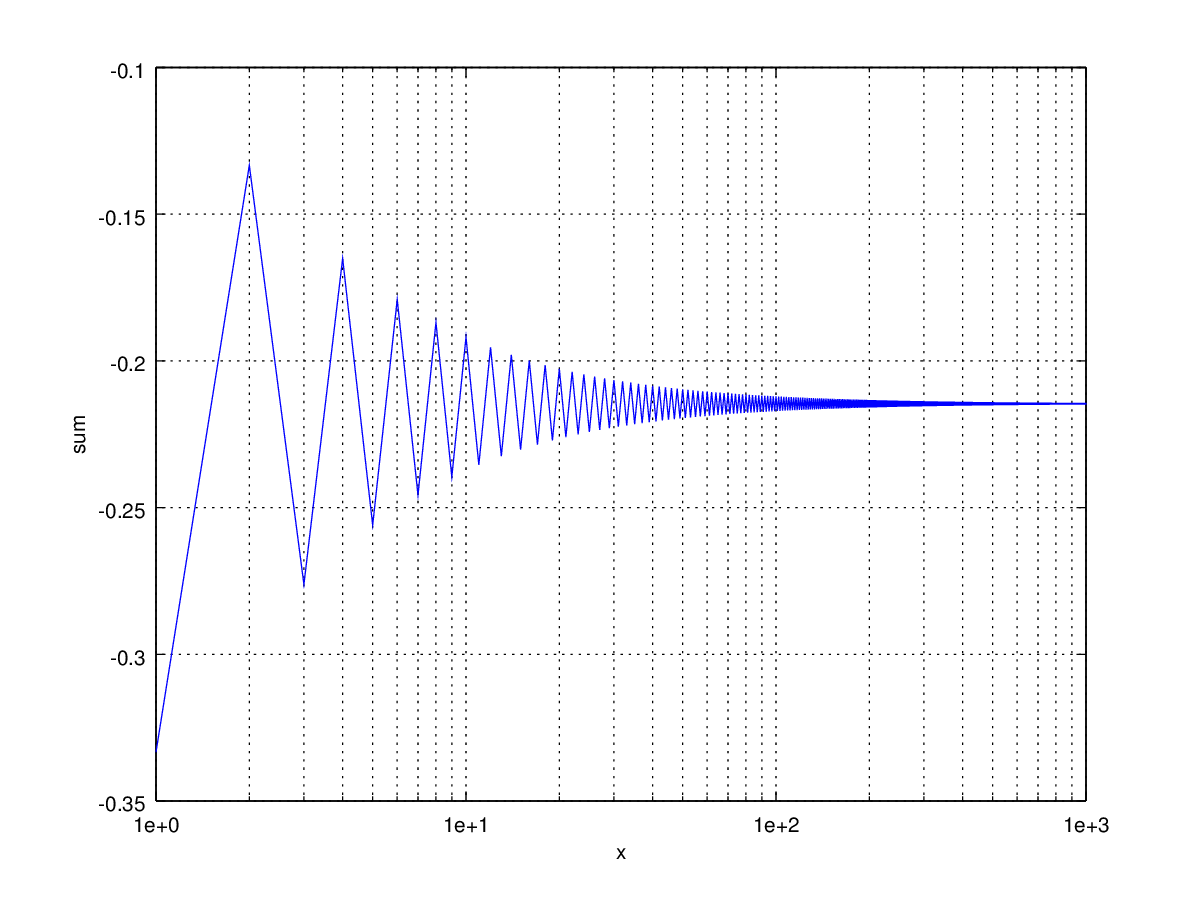
\includegraphics[width=\textwidth]{sum1.png}
	\end{minipage}
	\begin{minipage}[t]{0.5\textwidth}
		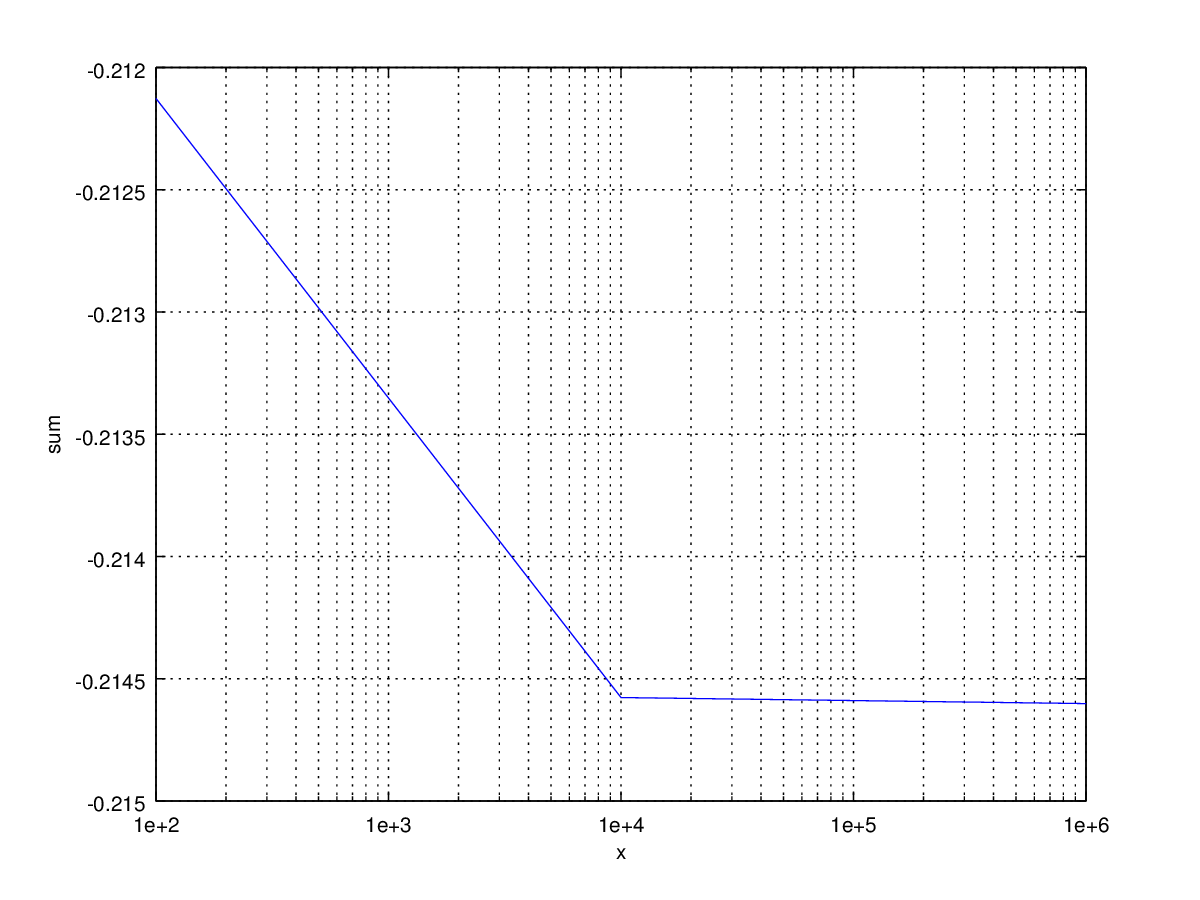
\includegraphics[width=\textwidth]{sum2.png}
	\end{minipage}
	\caption{sum calculation}
	\label{pic:sum}
\end{figure} 

\section*{3.) Picture puzzle}
\subsection*{a.)}


\subsection*{b.)}
\begin{figure}[htp!]
\begin{center}
	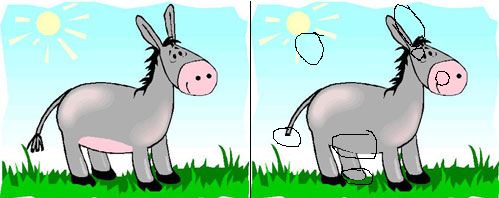
\includegraphics[scale=1.0]{esel_mistakes.png}
	\caption{marked mistakes}
\end{center}
\end{figure}
\newpage
\subsection*{c.)}
This code can count the mistakes of picture puzzle, if the pictures are the same in pixel by pixel without the mistakes.
\begin{Verbatim}[frame=bottomline]
	search.m
\end{Verbatim}

\VerbatimInput[frame=single]{search.m}%[firstline=3,lastline=5]

\section*{4.) gamma correction}
\subsection*{a.)}
A histogram is a diagram, which it can display the counts of pixels of every intensity level. The number of pixels are set it as x-axis and the intensity levels are set it as y-axis. Usually the number of pixels are display with vertical lines, but sometimes it is useful to use a bar plot for a better understanding. Also you can illustrate it as points or a single graph. For example a histogram of this picture (\ref{pic:hist_pic}).   

\begin{Verbatim}[frame=bottomline]
matlab_uebung_2_Ch.m
\end{Verbatim}
\VerbatimInput[firstline=1,lastline=5,frame=single]{matlab_uebung_2_Ch.m}

\begin{figure}[htp!]
	\begin{minipage}[t]{0.5\textwidth}
	\begin{center}
		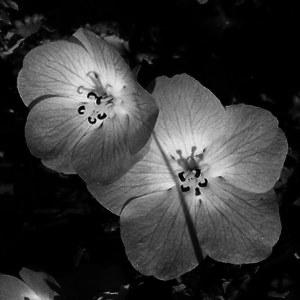
\includegraphics[scale=0.55]{flower.png}
	\end{center}
	\end{minipage}
	\begin{minipage}[t]{0.5\textwidth}
		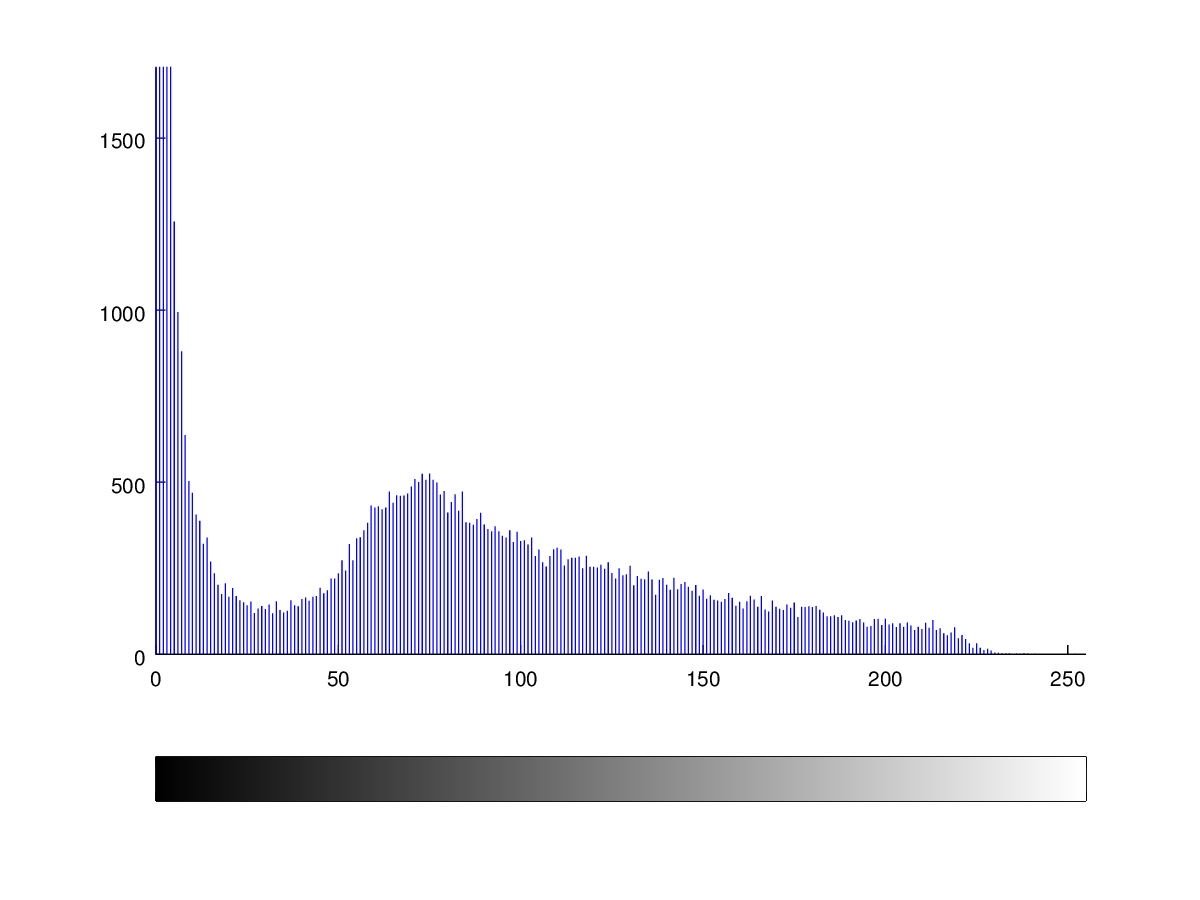
\includegraphics[scale=0.5]{histogram_flower.png}
	\end{minipage}
	\caption{histogram of a picture}
	\label{pic:hist_pic}
\end{figure}
\newpage
\subsection*{b.)}
The histgram equalization can performed with MATLAB commando 'histeq()' .

\VerbatimInput[firstline=6,lastline=9,frame=single]{matlab_uebung_2_Ch.m}%
%Kommandos

\begin{figure}[htp!]
	\begin{minipage}[t]{0.5\textwidth}
		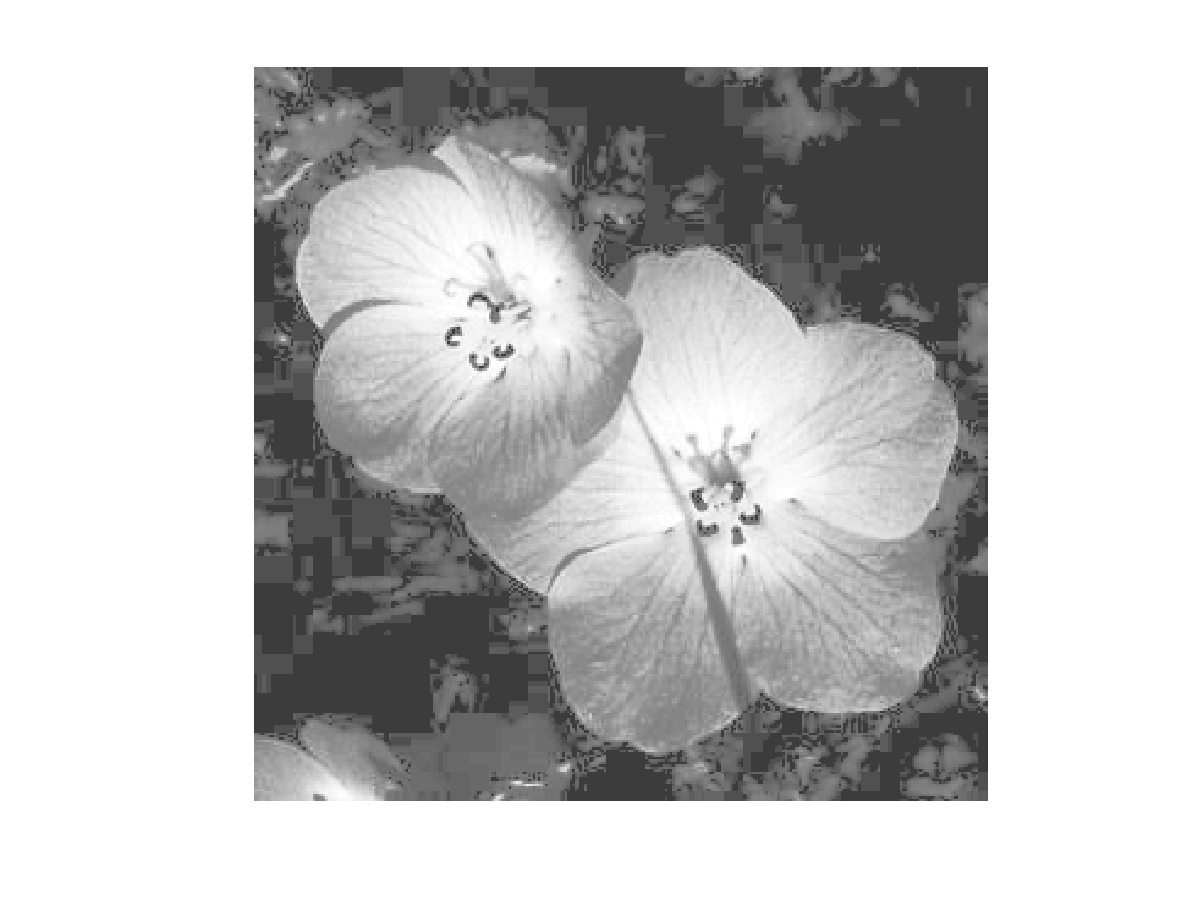
\includegraphics[width=\textwidth]{flower_eq.png}
	\end{minipage}
	\begin{minipage}[t]{0.5\textwidth}
		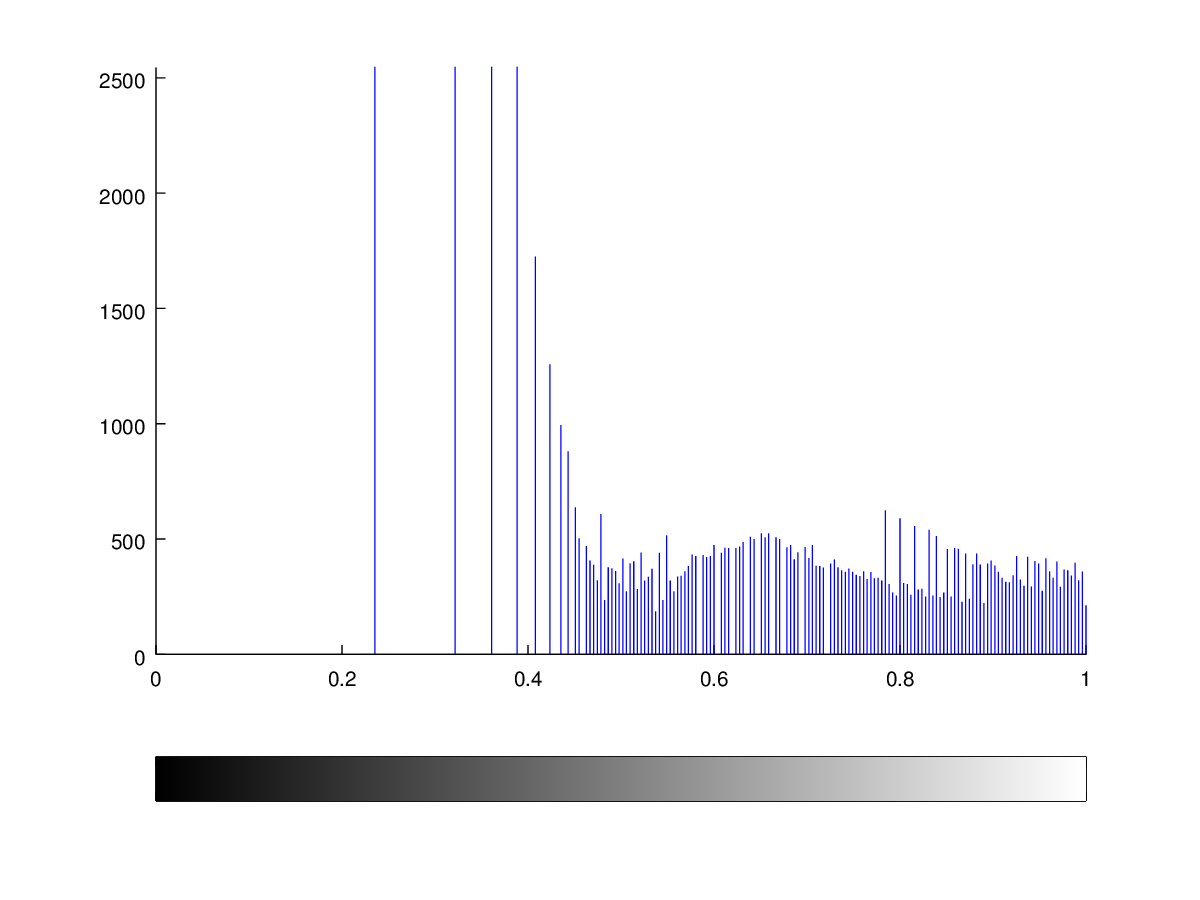
\includegraphics[width=\textwidth]{histoeq_flower.png}
	\end{minipage}
	\caption{histogram equalization of a picture}
	\label{pic:histoeq_pic}
\end{figure}

The transformation function can be find with these commandos.

\VerbatimInput[firstline=10,lastline=15,frame=single]{matlab_uebung_2_Ch.m}%
%Kommandos

\begin{figure}[htp!]
\begin{center}
	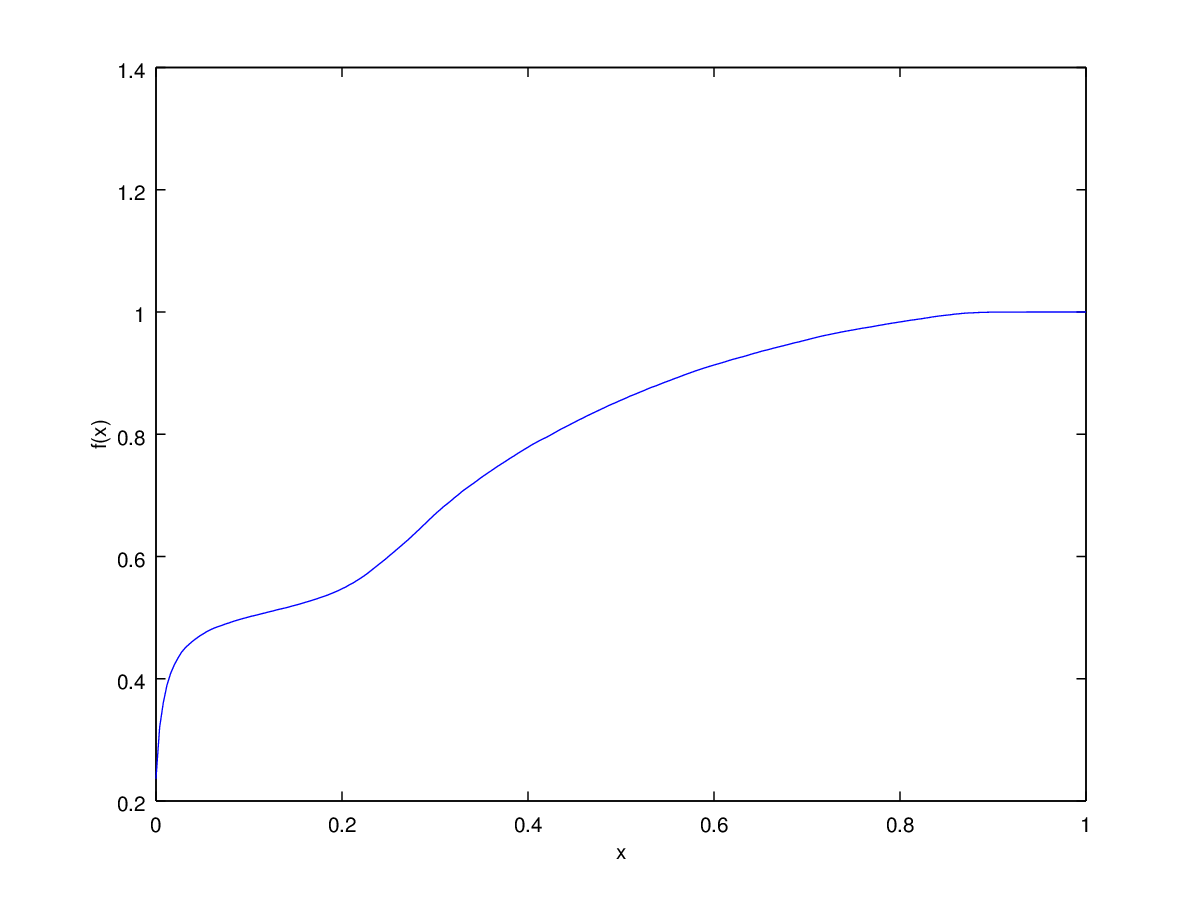
\includegraphics[scale=0.45]{histoeq_plot.png}
	\caption{plot of the transformation function $ f(x) $}
	%\label{pic:histoeq_plot}
\end{center}
\end{figure}

\subsection*{c.)}

\VerbatimInput[firstline=16,lastline=20,frame=single]{matlab_uebung_2_Ch.m}%
%Komandos

\begin{figure}[htp!]
	\begin{minipage}[t]{0.5\textwidth}
		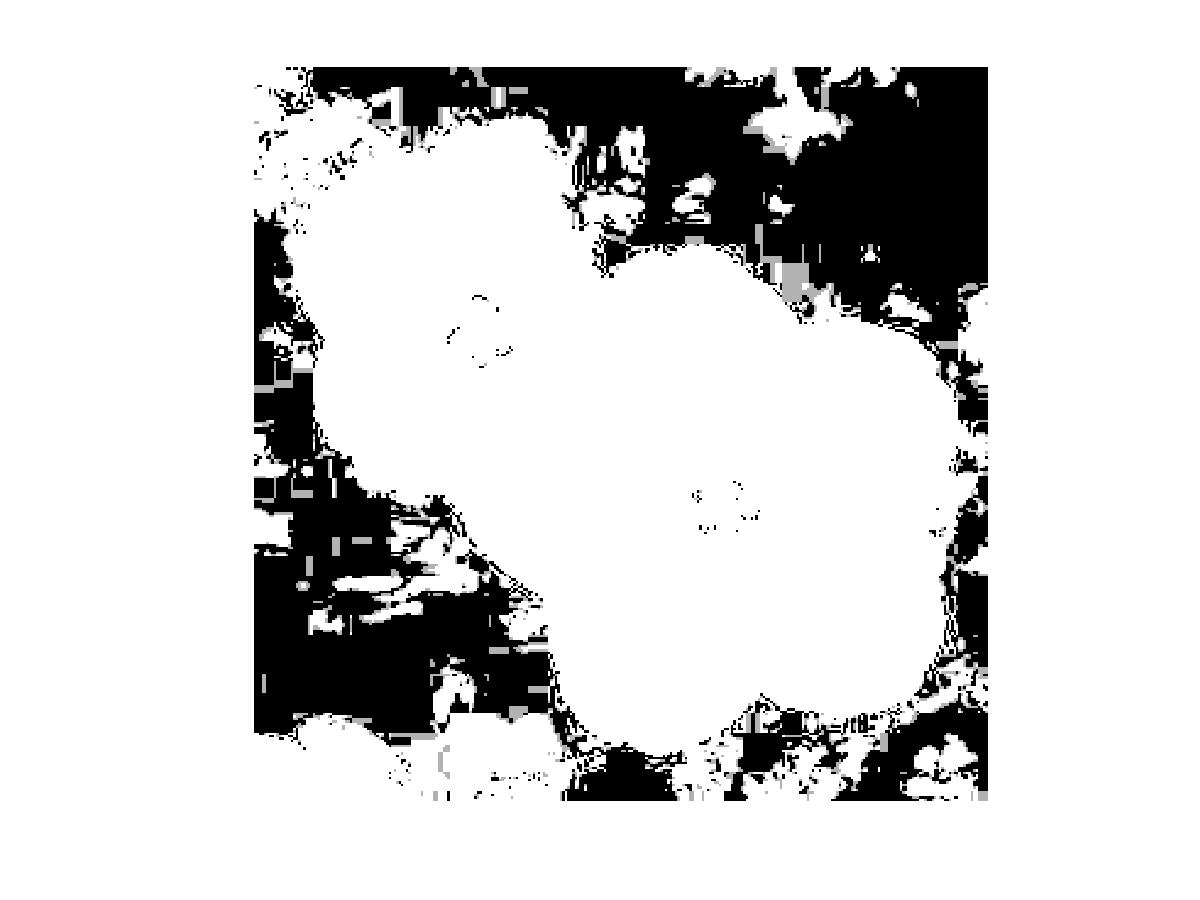
\includegraphics[width=\textwidth]{flower_low.png}
	\end{minipage}
	\begin{minipage}[t]{0.5\textwidth}
		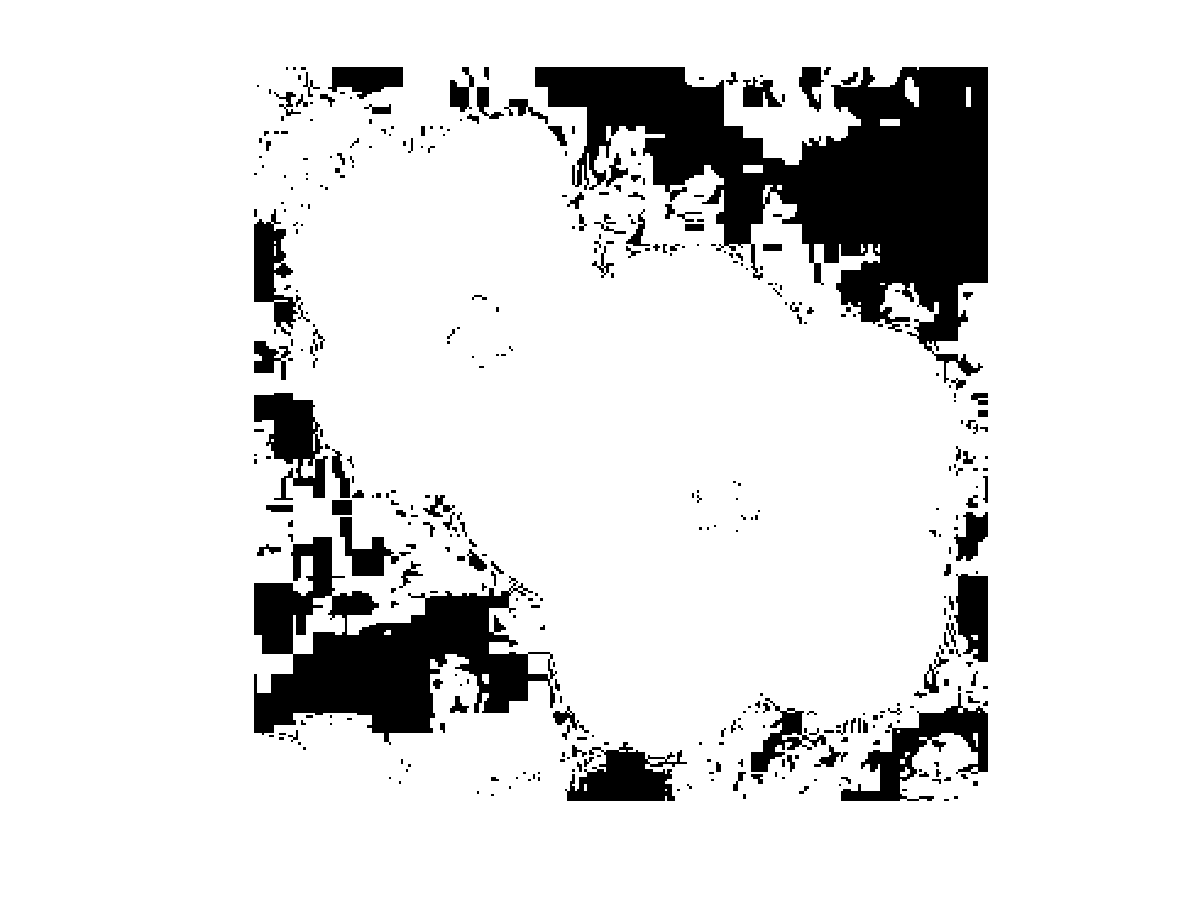
\includegraphics[width=\textwidth]{flower_high.png}
	\end{minipage}
	\caption{contrast enhancement by fraction of pixels in the lower (left) and higher (right) saturation region}
	%\label{pic:contrast_lohi}
\end{figure}

\subsection*{d.)}

\VerbatimInput[firstline=21,lastline=24,frame=single]{matlab_uebung_2_Ch.m}%
%Komanndos

\begin{figure}[htp!]
	\begin{minipage}[t]{0.5\textwidth}
		
\includegraphics[width=\textwidth]{flower_g1.png}
	\end{minipage}
	\begin{minipage}[t]{0.5\textwidth}
		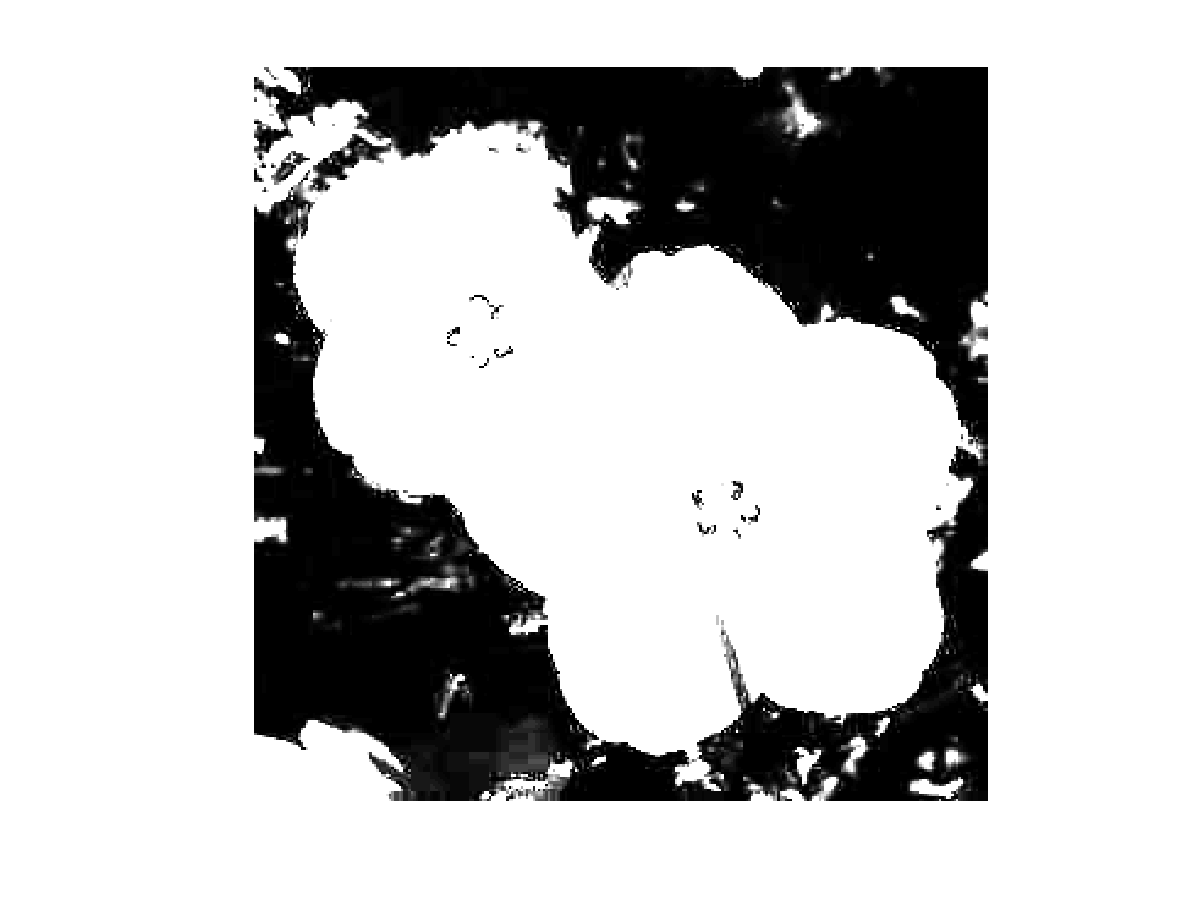
\includegraphics[width=\textwidth]{flower_g2.png}
	\end{minipage}
	\caption{gamma correction with $ \gamma = 0.5 $ (left) and $ \gamma = 2.0 $ (right)}
	%\label{pic:contrast_lohi}
\end{figure}

\subsection*{e.)}

\VerbatimInput[firstline=25,lastline=30,frame=single]{matlab_uebung_2_Ch.m}%
%Kommandos

\begin{figure}[htp!]
	\begin{minipage}[t]{0.5\textwidth}
		
\includegraphics[width=\textwidth]{flower_bin1.png}
	\end{minipage}
	\begin{minipage}[t]{0.5\textwidth}
		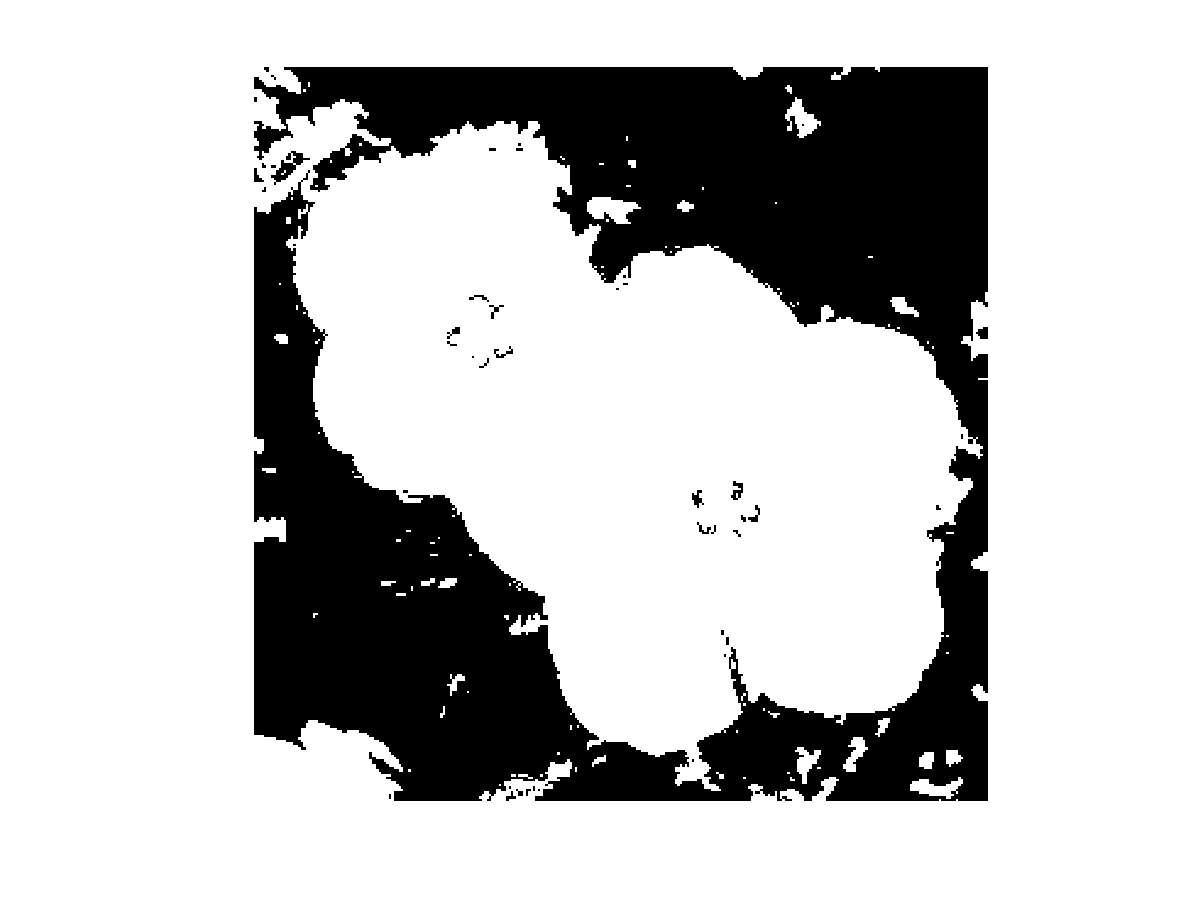
\includegraphics[width=\textwidth]{flower_bin2.png}
	\end{minipage}
	\caption{binary image before (left) and after (right) gamma correction with  $ \gamma = 2.0 $}
	%\label{pic:contrast_lohi}
\end{figure}

\subsection*{f.)}

\VerbatimInput[firstline=31,lastline=37,frame=single]{matlab_uebung_2_Ch.m}%
%Kommandos

\begin{figure}[htp!]
	\begin{minipage}[t]{0.3\textwidth}
		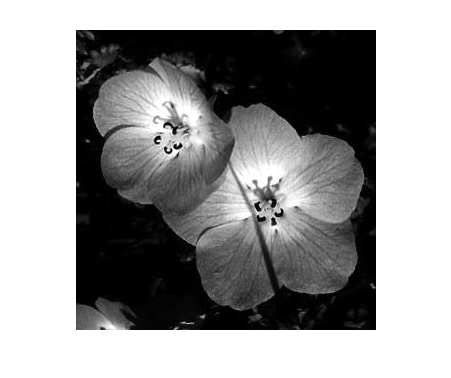
\includegraphics[width=\textwidth]{flower_imadjust.png}
	\end{minipage}
	\begin{minipage}[t]{0.3\textwidth}
		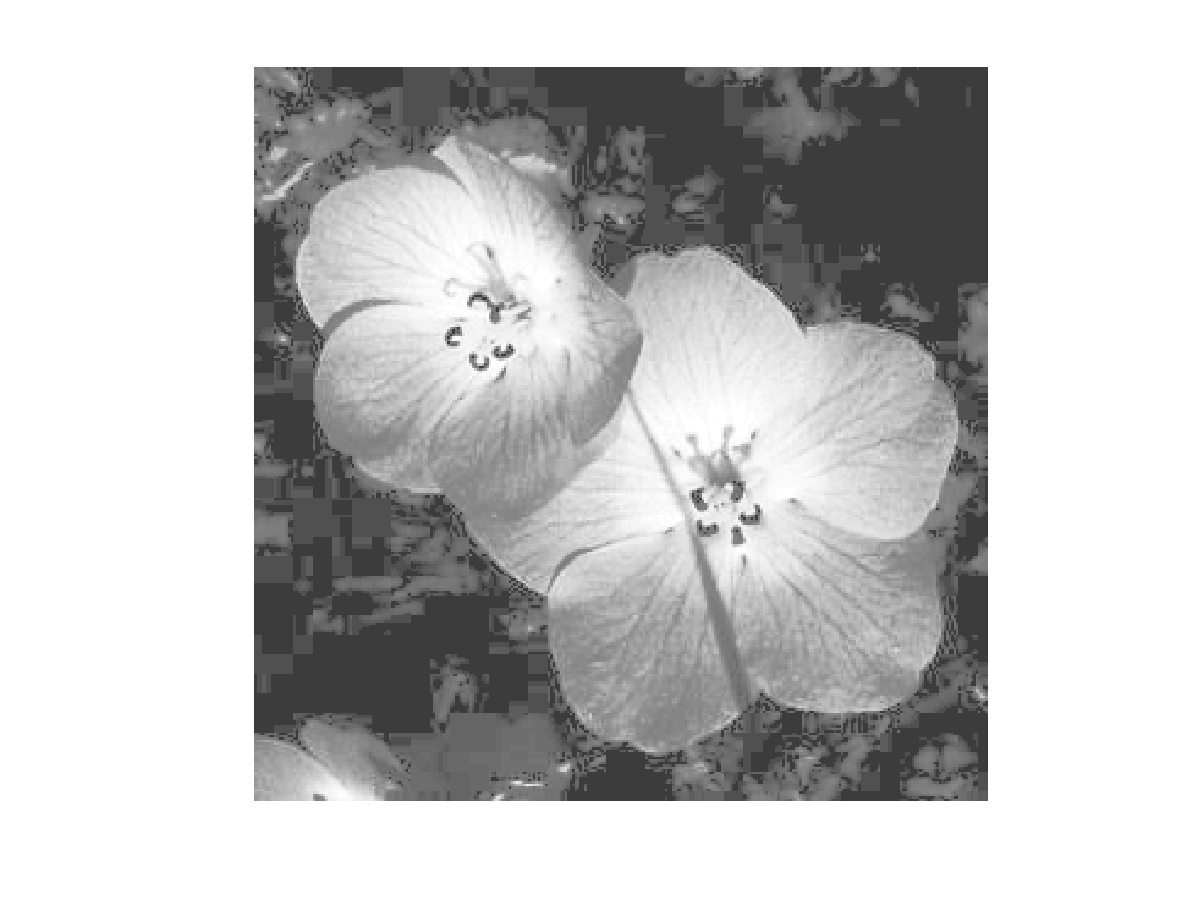
\includegraphics[width=\textwidth]{flower_eq.png}
	\end{minipage}
	\begin{minipage}[t]{0.3\textwidth}
		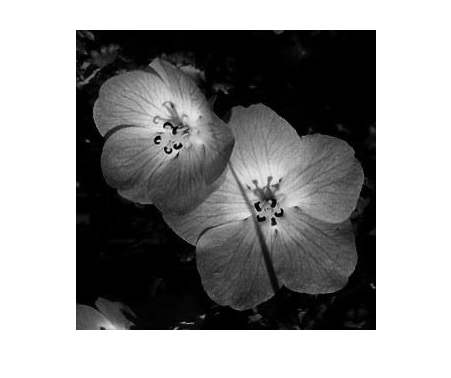
\includegraphics[width=\textwidth]{flower_adapt.png}
	\end{minipage}
	\caption{function imadjust (left), histeq (mid) and adapthisteq (right)}
	%\label{pic:contrast_lohi}
\end{figure}


\begin{comment}

\begin{alltt}
\input{distance.m}
\end{alltt}

\begin{Verbatim}
hhhhhhhh dcdf cf fvv v fv 
\end{Verbatim}
\end{comment}

\end{document}
